\documentclass[12pt, a4paper]{ctexart}
\usepackage{amsmath, amssymb, amsfonts}
\usepackage{graphicx}
\usepackage{booktabs}
\usepackage{geometry}
\usepackage{hyperref}

\geometry{left=2.5cm, right=2.5cm, top=2.5cm, bottom=2.5cm}

\begin{document}

\begin{abstract}
全文最后写。三句话套路:方法 / 核心 / 量化结果。必须贴 3 张 Q1/Q2/Q3 缩略图。 关键词:柱面反射变形、几何光学、逆问题、反向光线追踪、兼容性判据、Catoptric Anamorphosis
\end{abstract}

\section{问题重述与研究背景}

\subsection{研究背景}
变形艺术(Anamorphosis)是一类基于几何畸变的视觉艺术形式,其特点是:在常规观察条件下,图像呈现无法识别的扭曲形态;仅当观察者处于特定空间位置,或借助特定光学介质(如反射镜)时,图像才会还原为可辨认的内容。该艺术形式的发展贯穿了文艺复兴以来的西方艺术史,同时也催生了一系列几何学与光学的数学研究。

从历史脉络看,变形艺术经历了从平面斜视畸变(Oblique Anamorphosis)向曲面反射畸变(Catoptric Anamorphosis)的演变。列奥纳多·达·芬奇在《大西洋古抄本》(Codex Atlanticus, 1483–1518)中绘制了已知最早的变形手稿。16世纪,平面斜视畸变被广泛运用于隐喻性图像的创作,汉斯·荷尔拜因于1533年创作的油画《大使们》(The Ambassadors)是其中的代表作——画作底部的模糊条状图形在特定的斜视角度下呈现为完整的人类头骨。16世纪末至17世纪,变形艺术的载体由平面空间转向曲面光学介质,柱面与锥面镜反射畸变开始流行。1638年,法国数学家让-弗朗索瓦·尼塞龙(Jean-François Nicéron)出版专著《奇妙的透视》(La perspective curieuse),系统阐述了柱面、锥面镜变形图案的几何作图法,提出了基于网格变换的构造方案,为该领域的数学化研究奠定了文献基础。

在数学研究层面,针对柱面镜变形的定量建模自20世纪起逐步成熟。Hunt、Nickel 与 Gigault 于2000年在《American Journal of Physics》发表的 Anamorphic Images 一文中,推导了有限观察距离与观察高度条件下,目标平面坐标与纸面畸变坐标之间的非线性代数变换方程,并给出了观察者位于无穷远处时的线性退化形式。Spickler 与 Bergner 在2011年进一步给出了基于三维向量代数的六步正向光线追踪模型,将反射定律与柱面几何方程联立求解,为算法化求解提供了可操作的数学框架。近年来,该问题在计算机图形学领域得到进一步发展:Geng 等人于 CVPR 2024 提出的 Visual Anagrams 利用扩散模型生成多视角光学错觉图像,计算生成方法正在拓展变形艺术的设计边界。

在现代艺术与商业领域,柱面变形作为独立的视觉媒介被持续应用。当代艺术家 Reza Ezoji 借助实体的圆柱形钢镜,通过实时观察镜面反射进行逆向手绘,创作了大量具象肖像作品。韩国 Luycho 公司于2013年推出的 Mirror Cup \& Saucer 系列,将该原理应用于消费产品——表面镀金或镀铂的陶瓷杯与印有畸变图案的茶托相配合,观察者将杯子置于茶托中心时,畸变图形被反射为可辨识的图像。该系列已发展出濒危动物、仿 Eadweard Muybridge 摄影的 Locomotion 等多个主题,展示了数学原理在艺术产品中的商业化潜力。

\subsection{问题重述}
本文以柱面镜变形艺术的数学建模为研究对象。假设纸张为理想平面上的 A4 幅面区域,镜面为理想圆柱体侧面且竖直放置。定义纸张上绘制的图案为纸面图案,观察者通过圆柱镜面看到的反射图案为镜面图案。在此背景下,本文需要解决以下三个问题:

\textbf{问题一:}给定特定的镜面图案参考图,建立从镜面图案反推纸面图案的数学模型,并同步确定圆柱镜面的几何参数(半径、高度)与摆放位置等。要求针对题目附图 3(蒙娜丽莎肖像)与附图 4(卡通猫形象)给出具体的设计方案,包括纸面图案、镜面几何尺寸与观察视点的完整数值结果。

\textbf{问题二:}探讨纸面图案本身是否可以承载独立艺术意义。该问题分为两个子情形:
\begin{itemize}
    \item \textbf{子问题 (a):}在不指定镜面图案的条件下,能否设计出纸面图案与镜面图案均有意义的作品?两者的内容可以独立,不要求存在关联。
    \item \textbf{子问题 (b):}在指定镜面图案的条件下,能否设计出纸面图案同样具有艺术意义的作品?
\end{itemize}

\textbf{问题三:}若同时指定任意的镜面图案与纸面图案,仅通过艺术加工,能否设计出两者均有意义的作品?本文需要探讨当要求镜面图案与纸面图案均有意义时,两者在几何、拓扑、频域等层面所应满足的兼容性条件或关系,并给出相应的判别方法。

三个问题呈递进关系:问题一建立基础的正向/逆向映射模型,属于确定性求解;问题二在保留部分自由度的前提下引入双重艺术约束,属于构造性设计;问题三在完全约束条件下讨论可行性边界,属于开放性的理论判据问题。本文将依次展开相应的建模、算法与案例分析。

\subsection{研究思路概览}
一段话串起 Q1$\rightarrow$Q2$\rightarrow$Q3 的逻辑。配一张总流程图。


\section{符号与数学框架总论}
\subsection{基本假设}

为便于数学建模与分析,本文做出以下基本假设。每条假设均说明其合理性,对于在后续章节中松绑或深化的假设,本节亦作简要说明。

\textbf{假设 1(纸张理想化):} 纸张视为 $xy$ 平面( $z=0$ )上的理想矩形区域,尺寸为 $L_{A4} \times W_{A4} = 297 \times 210$ mm。纸张不发生弯曲、褶皱或形变。

\textbf{合理性:} A4 纸在实际使用中以平整状态置于桌面,厚度约 0.1 mm,远小于镜面半径 $R$ (典型值 20–50 mm),平面化假设误差可忽略。

\textbf{假设 2(镜面理想化):} 圆柱镜面为理想光滑曲面,反射率为 100\%,镜面本身无厚度。圆柱轴竖直(平行于 $z$ 轴),底面圆心位于纸面上的 $(x_0, y_0)$ 处,半径为 $R$ ,高度为 $H$ 。

\textbf{合理性:} 实际抛光金属镜面反射率可达 90\% 以上,100\% 假设不改变反射路径的几何结果,仅影响图像亮度。镜面厚度在商业产品中约 1–2 mm,相对于 $R$ 为高阶小量,忽略后不影响映射的几何形态。

\textbf{假设 3(镜面不透明):} 圆柱镜为实体,观察者无法穿过镜面观察其背后的纸面区域。纸面上被圆柱底面所覆盖的圆盘区域 $\{(u, v) : (u-x_0)^2 + (v-y_0)^2 \leq R^2\}$ 不参与反射,亦不被观察者直接看到。

\textbf{合理性:} 符合物理直觉与实际作品的观察条件。该假设对于 Q2(b) 中可视盲区的几何推导至关重要。

\textbf{假设 4(观察者模型:Q1 单点视点,Q2/Q3 可拓展至双眼视差):} 在 Q1 的基础建模中,观察者视为空间中的单点 $\mathbf{E} = (x_E, y_E, z_E)$ ,忽略双眼视差;在 Q2 与 Q3 的讨论中,可在单点模型基础上引入双眼视差、清晰视区与舒适视区等人眼感知因素作为修正项。

\textbf{合理性:} 实际观察时双眼瞳距约 65 mm,典型观察距离 $D \geq 500$ mm,视差角不超过 $7.5^\circ$ ;对于 Q1 的几何映射精度而言,单点假设误差位于图像分辨率以下,可忽略。对于高质量艺术效果,双眼观察到的镜面图案需具备近似一致的虚像深度,以避免复视,这一讨论在后续章节展开。

\textbf{假设 5(几何光学反射定律):} 光在镜面上的传播遵循几何光学反射定律——入射光线、反射光线与反射点处的曲面法向量共面,且入射角与反射角相等。忽略光的波动性、衍射、偏振效应。

\textbf{合理性:} 可见光波长(400–700 nm)远小于镜面几何尺度(毫米级),衍射效应可忽略,几何光学近似成立。

\textbf{假设 6(一次反射):} 仅考虑入射光线与镜面的一次反射,忽略镜面多次内反射、边缘绕射,以及纸面的漫反射回到镜面再反射的二次成像。

\textbf{合理性:} 圆柱镜面为凸面,单次反射已将光线发散至远方,二次反射返回观察者视线的概率极低,其贡献在亮度上位于背景噪声量级。

\textbf{假设 7(图像离散化误差可控):} 纸面图案与镜面图案均视为理想的连续二维函数 $F(u, v)$ 与 $G(\theta, z)$ ,离散化误差仅来自数值渲染的分辨率选择。

\textbf{合理性:} 通过选取足够高的分辨率(如 300 DPI,对应像素步长 $a \approx 0.085$ mm),离散化误差小于人眼可辨识阈值。

\textbf{假设 8(印刷与材料理想化):} 不考虑油墨厚度、纸张的反光性、打印颜色偏差以及镜面的轻微色散。纸面图案的呈现与数学模型输出完全一致。

\textbf{合理性:} 上述物理因素影响最终作品的视觉质量,但不影响映射的几何结构。相关工程修正超出本文数学建模的讨论范围。

\textbf{假设 9(观察环境理想化):} 观察环境光照充足且均匀,不考虑阴影、环境光遮挡、镜面污渍等外部扰动。

\textbf{合理性:} 本文关注几何映射本身,环境因素属于作品展示条件,不影响数学建模结论。

\textbf{小结:} 上述 9 条假设中,假设 1–3、5–9 在全文各问题中保持一致;假设 4 在 Q1 中采用简化形式,并在 Q2、Q3 的高质量设计讨论中进一步拓展,以体现本文模型对真实观察条件的适应性。

\subsection{符号说明}

\subsubsection*{全局约定}
\begin{itemize}
    \item 长度单位:全部使用 mm(A4 = 297 $\times$ 210 mm)
    \item 角度单位:全部使用 rad
    \item 坐标系层级(四套,各有用途):
\end{itemize}

\begin{table}[htbp]
\centering
\begin{tabular}{ll}
\toprule
\textbf{坐标系} & \textbf{使用场景} \\
\midrule
3D 直角坐标 (x, y, z) & 光线追踪、反射定律、向量运算 \\
镜面柱面参数 ($\theta$, z) & 镜面离散化、镜面图像存储 \\
纸面极坐标 ($\rho$, $\phi$) & 对称性分析、FFT、Q2/Q3 兼容性判据 \\
纸面直角坐标 (u, v) & A4 打印输出、像素位图存储 \\
\bottomrule
\end{tabular}
\end{table}

\subsubsection*{1. 几何参数}
\begin{table}[htbp]
\centering
\begin{tabular}{lllp{6cm}}
\toprule
\textbf{符号} & \textbf{含义} & \textbf{单位} & \textbf{备注} \\
\midrule
$R$ & 圆柱镜面半径 & mm & 典型值 20–50 \\
$H$ & 圆柱镜面高度 & mm & 典型值 90–150 \\
$(x_0, y_0)$ & 圆柱底面中心在纸面上的投影坐标 & mm & 默认 $(0, 0)$ \\
$L_{A4}$ & A4 纸张长边 & mm & $L_{A4} = 297$ \\
$W_{A4}$ & A4 纸张短边 & mm & $W_{A4} = 210$ \\
\bottomrule
\end{tabular}
\end{table}

\subsubsection*{2. 观察者}
\begin{table}[htbp]
\centering
\begin{tabular}{lllp{5cm}}
\toprule
\textbf{符号} & \textbf{含义} & \textbf{单位} & \textbf{备注} \\
\midrule
$\mathbf{E} = (0, D, z_E)$ & 观察者视点 3D 位置（MATLAB 坐标约定） & mm & 单点视点假设 \\
$D$ & 观察者到圆柱轴（$z$ 轴）的水平距离 & mm & 对称放置下 $D = y_E$，标量 \\
$z_E$ & 观察者视点高度 & mm & $z_E > 0$，本文取 $350$ mm \\
\bottomrule
\end{tabular}
\end{table}

\subsubsection*{3. 镜面参数化与 3D 坐标}
\begin{table}[htbp]
\centering
\begin{tabular}{lllp{6cm}}
\toprule
\textbf{符号} & \textbf{含义} & \textbf{单位} & \textbf{备注} \\
\midrule
$\theta$ & 镜面上点的方位角 & rad & $\theta \in [0, 2\pi)$ \\
$z$ & 镜面上点的高度 & mm & $z \in [z_{\min}, z_{\max}] \subseteq [0, H]$ \\
$z_{\min}, z_{\max}$ & 镜面图像垂直方向的高度区间 & mm & $z_{\max} - z_{\min} \leq H$ \\
$[\theta_1, \theta_2]$ & 镜面图像所占的方位角区间 & rad & 通常取对称区间 \\
$\mathbf{P}_{mirror}$ & 镜面上点的 3D 直角坐标 & mm & $x = x_0 + R\sin\theta,$ \newline $y = y_0 + R\cos\theta$ \\
$\mathbf{n}$ & 镜面点处的外法向量 & — & $\mathbf{n} = (\sin\theta, \cos\theta, 0)$ \\
\bottomrule
\end{tabular}
\end{table}

\subsubsection*{4. 光线追踪向量}
\begin{table}[htbp]
\centering
\begin{tabular}{lllp{6cm}}
\toprule
\textbf{符号} & \textbf{含义} & \textbf{单位} & \textbf{备注} \\
\midrule
$\mathbf{d}$ & 入射方向向量 & — & $\mathbf{d} = (\mathbf{P}_{mirror} - \mathbf{E}) / \lVert \cdot \rVert$ \\
$\mathbf{r}$ & 反射方向向量 & — & $\mathbf{r} = \mathbf{d} - 2(\mathbf{d}\cdot\mathbf{n})\mathbf{n}$ \\
$t^*$ & 反射线与 $z=0$ 平面交点参数 & — & $\mathbf{P}_{mirror} + t\mathbf{r}$ 令 $z=0$ \\
\bottomrule
\end{tabular}
\end{table}

\subsubsection*{5. 纸面坐标(双表示)}
\begin{table}[htbp]
\centering
\begin{tabular}{lllp{6cm}}
\toprule
\textbf{符号} & \textbf{含义} & \textbf{单位} & \textbf{备注} \\
\midrule
$(s, t)$ & 虚拟视平面局部坐标（仅 Q1 实现用） & mm & $s$ 水平、$t$ 垂直；代表参考图 $G_{\mathrm{ref}}$ 上的像素位置 \\
$(u, v)$ & 纸面直角坐标 & mm & 原点在 $(x_0, y_0)$，用于 A4 打印输出 \\
$(\rho, \phi)$ & 纸面极坐标 & mm/rad & 原点在 $(x_0, y_0)$，$\phi = 0$ 指向观察者投影方向 \\
$\mathbf{P}_{\mathrm{paper}}$ & 纸面对应点 & mm & $= (u, v, 0)$ 或等价表示 $(\rho, \phi)$ \\
$\rho_{\min}, \rho_{\max}$ & 可视环形区域的内、外半径 & mm & 由观察者位置与 $R, H$ 决定 \\
$I_{\mathrm{vis}}$ & 纸面可视环形区域 & --- & $\{(\rho, \phi) : \rho_{\min} \leq \rho \leq \rho_{\max}\}$ 的子集 \\
\bottomrule
\end{tabular}
\end{table}

\subsubsection*{6. 映射与图像函数}
\begin{table}[htbp]
\centering
\begin{tabular}{lll}
\toprule
\textbf{符号} & \textbf{含义} & \textbf{备注} \\
\midrule
$T$ & 正向映射：纸面 $\rightarrow$ 镜面 & $T: (u, v) \mapsto (\theta, z)$ \\
$T^{-1}$ & 逆向映射：镜面 $\rightarrow$ 纸面 & $T^{-1}: (\theta, z) \mapsto (u, v)$，本文核心算子 \\
$F(u, v)$ 或 $F(\rho, \phi)$ & 纸面图案函数 & 值域为灰度 $[0, 1]$ 或 RGB \\
$G(\theta, z)$ & 镜面图案函数 & 值域同上 \\
$\hat{G} = F \circ T^{-1}$ & 纸面图案在镜面上的反射结果 & 用于和目标图案 $G$ 对比 \\
\bottomrule
\end{tabular}
\end{table}

\subsubsection*{7. 离散化与像素}
\begin{table}[htbp]
\centering
\begin{tabular}{lllp{6cm}}
\toprule
\textbf{符号} & \textbf{含义} & \textbf{单位} & \textbf{备注} \\
\midrule
$a$ & 像素物理尺寸步长 & mm & 300 DPI 时约 $0.0847$ \\
$M, N$ & 镜面像素矩阵的行、列数 & — & $M = (z_{\max}-z_{\min})/a,$ \newline $N = R(\theta_2-\theta_1)/a$ \\
$S_{M \times N}$ & 镜面图像像素矩阵 & — & 存储色彩或灰度信息 \\
$(i, j)$ & 像素矩阵的行列下标 & — & $i \in [0, M),\; j \in [0, N)$ \\
\bottomrule
\end{tabular}
\end{table}

\subsubsection*{8. Q3 兼容性分析专用}
\begin{table}[htbp]
\centering
\begin{tabular}{lll}
\toprule
\textbf{符号} & \textbf{含义} & \textbf{备注} \\
\midrule
$D_{\text{diff}}$ & 差异图 $G - T(F)$ & 用于衡量纸面与镜面不兼容程度 \\
$\varepsilon_1, \dots, \varepsilon_5$ & 兼容性判据阈值 & 拓扑 / 尺度 / 对称 / 可视 / 容忍度 \\
$\mathcal{F}_{polar}(F)$ & 极坐标下的 2D FFT & 角频谱 + 径频谱 \\
$\mathcal{F}_{cart}(G)$ & 镜面图案的 2D FFT & 横频谱 + 纵频谱 \\
\bottomrule
\end{tabular}
\end{table}

\subsection{坐标系选择与对比}

\subsubsection{四套坐标系的功能分层}

本文涉及的建模任务横跨三维空间几何、曲面离散化与二维打印输出三个层面，任何单一坐标系均难以同时兼顾全部需求。为此，本文采用四套坐标系分层配合的方案：3D 直角坐标 $(x,y,z)$ 用于光线追踪与反射定律的向量推导；镜面柱面参数坐标 $(\theta,z)$ 用于镜面的均匀离散化与图案存储；纸面极坐标 $(\rho,\phi)$ 用于揭示圆对称性、支撑 Q2/Q3 中的兼容性分析；纸面直角坐标 $(u,v)$ 用于最终的 A4 打印输出与像素位图生成。各坐标系各司其职，通过映射算子 $T$ 与 $T^{-1}$ 相互衔接，共同构成完整的建模框架。

\subsubsection{镜面参数化的选择}

若以 3D 直角坐标 $(x,y,z)$ 描述镜面上的点，则每个点须满足隐式约束 $x^2+y^2=R^2$，三个坐标分量之间存在非线性耦合，采样与插值操作均需额外处理。柱面参数坐标 $(\theta,z)$ 是圆柱面的无冗余自然参数化：给定 $(\theta,z)$，镜面点的 3D 坐标由
\[
\mathbf{P}_{\mathrm{mirror}}=\bigl(x_0+R\sin\theta,\;y_0+R\cos\theta,\;z\bigr)
\]
唯一确定，无需附加约束。此外，$(\theta,z)$ 矩形网格直接对应圆柱面的展开图，镜面图案函数 $G(\theta,z)$ 可按标准位图格式存储与检索，便于后续的插值与渲染操作。

\subsubsection{纸面坐标的双表示}

纸面采用直角坐标 $(u,v)$ 与极坐标 $(\rho,\phi)$ 的双表示，各有其不可替代的优势。$(u,v)$ 与像素坐标直接对应，是打印输出的必要形式。$(\rho,\phi)$ 则天然适配圆柱镜在纸面形成的环形可视区域 $I_{\mathrm{vis}}$，便于描述内外半径约束 $\rho_{\min}\leq\rho\leq\rho_{\max}$。

更为关键的是，极坐标揭示了一条重要的对称性规律：纸面极角 $\phi$ 与镜面方位角 $\theta$ 之间存在近似单调映射，纸面径向距离 $\rho$ 则主要由镜面高度 $z$ 决定。这意味着，纸面上的放射状图案（$\phi$ 方向变化）对应镜面上的竖条纹（$\theta$ 方向变化），纸面上的同心圆图案（$\rho$ 方向变化）对应镜面上的横条纹（$z$ 方向变化）。这一对称性观察是后续 FFT 兼容性判据的数学基础。

\subsubsection{反射映射在不同坐标系下的表达对比}

同一反射映射在不同坐标系下的表达复杂度差异显著，如表~\ref{tab:coord-compare} 所示。

\begin{table}[htbp]
\centering
\caption{反射映射在不同坐标系下的计算复杂度对比}
\label{tab:coord-compare}
\begin{tabular}{llll}
\toprule
\textbf{映射方向} & \textbf{坐标系} & \textbf{计算方式} & \textbf{详见} \\
\midrule
$(\theta,z)\to(u,v)$ & 柱面$\to$直角 & 完整光线追踪向量运算，无解析捷径 & 第 2.4.1 节 \\
$(\theta,z)\to(\rho,\phi)$ & 柱面$\to$极坐标 & 基于 Hunt et al.（2000）的显式代数近似 & 第 2.4.2 节 \\
$(u,v)\to(\theta,z)$ & 直角$\to$柱面 & 需求解关于 $\theta$ 的非线性方程组 & 第 2.4.3 节 \\
\bottomrule
\end{tabular}
\end{table}

由此可见，极坐标下的正向映射具有最简洁的解析结构，适合参数确定与对称性分析；直角坐标下的逆向映射则是图像生成的最终形式。实际计算中应根据任务需要选择最方便的坐标系，而非一律使用同一表示。

\subsection{圆柱镜面反射的几何映射模型}

为系统描述纸面图案与镜面图案之间的关系，本文建立正向映射 $T$ 与逆向映射 $T^{-1}$，并在不同坐标系下给出其数学表达。映射算子定义为：
\[
T:(u,v)\mapsto(\theta,z),\qquad T^{-1}:(\theta,z)\mapsto(u,v).
\]

\subsubsection{基于镜面参数坐标 $(\theta,z)$ 的映射模型（核心）}

镜面上的点参数化为：
\[
\mathbf{P}_{\mathrm{mirror}}(\theta,z)=\bigl(x_0+R\sin\theta,\;y_0+R\cos\theta,\;z\bigr).
\]
单位外法向量为 $\mathbf{n}(\theta)=(\sin\theta,\cos\theta,0)$。

逆向映射（由镜面到纸面）是本文核心算子。从观察者 $\mathbf{E}$ 出发，经镜面点 $\mathbf{P}_{\mathrm{mirror}}(\theta,z)$ 反射后与纸面 $z=0$ 相交于纸面点 $\mathbf{P}_{\mathrm{paper}}=(u(\theta,z),v(\theta,z),0)$。令入射视线单位向量
\[
\mathbf{d}=\frac{\mathbf{P}_{\mathrm{mirror}}-\mathbf{E}}{\lVert\mathbf{P}_{\mathrm{mirror}}-\mathbf{E}\rVert},
\]
根据反射定律，反射方向向量 $\mathbf{r}$ 满足：
\[
\mathbf{r}(\theta,z)=\mathbf{d}-2\bigl(\mathbf{d}\cdot\mathbf{n}(\theta)\bigr)\,\mathbf{n}(\theta).
\]
参数方程 $P(t)=\mathbf{P}_{\mathrm{mirror}}+t\mathbf{r}$ 与平面 $z=0$ 求交，得：
\[
t(\theta,z)=-\frac{z}{r_z(\theta,z)},\quad(t>0,\;r_z<0).
\]
则逆向映射为：
\[
T^{-1}(\theta,z)=\bigl(u(\theta,z),\;v(\theta,z)\bigr)=\mathbf{P}_{\mathrm{mirror}}(\theta,z)+t(\theta,z)\cdot\mathbf{r}(\theta,z).
\]
纸面图案可由 $F\bigl(T^{-1}(\theta,z)\bigr)=G(\theta,z)$ 确定。

\textbf{可见性约束}：上述逆向映射仅对可见镜面点有效，需同时满足：
\[
\mathbf{d}\cdot\mathbf{n}(\theta)<0\quad\text{（镜面点位于观察者可见侧）},\qquad r_z<0\quad\text{（反射线向下与纸面相交）}.
\]
不满足上述条件的镜面点予以剔除，不参与图案生成。

\subsubsection{基于纸面极坐标 $(\rho,\phi)$ 的映射模型}

\textbf{对称放置假设}：约定观察者位于 $y$ 正半轴方向，即 $\mathbf{E}=(0,D,z_E)$，$\phi=0$ 方向指向观察者投影方向。

以圆柱轴心 $(x_0,y_0)$ 为极点建立纸面极坐标 $(\rho,\phi)$。基于 Hunt et al.（2000）针对柱面镜提出的代数映射模型，定义中间系数（完整推导详见附录）：
\[
\alpha(z)=\frac{z_E-2z}{z_E-z},\qquad\beta(z)=\frac{z}{z_E-z},
\]
则纸面极坐标下的正向映射满足：
\[
\rho(\theta,z)=\sqrt{\alpha(z)^2R^2+\beta(z)^2D^2+2\alpha(z)\beta(z)RD\cos\theta},
\]
\[
\phi(\theta,z)=\operatorname{atan2}\!\bigl(\alpha(z)R\sin\theta+\beta(z)D\sin2\theta,\;\alpha(z)R\cos\theta+\beta(z)D\cos2\theta\bigr).
\]
该映射关于 $\theta=0$ 对称，在 $z<z_E$ 时光滑。逆向映射 $T^{-1}$ 在极坐标下无简洁解析式，通常通过数值方法由 $(\rho,\phi)$ 反求 $(\theta,z)$。

\subsubsection{基于纸面直角坐标 $(u,v)$ 的映射模型}

正向映射 $T:(u,v)\mapsto(\theta,z)$ 可通过求解以下非线性方程组获得：
\[
\begin{cases}
(x_0+R\sin\theta-u)^2+(y_0+R\cos\theta-v)^2=R^2,\\
\text{反射定律约束条件.}
\end{cases}
\]
逆向映射 $T^{-1}:(\theta,z)\mapsto(u,v)$ 则通过第 2.4.1 节中的向量形式直接计算，得到 $(u,v)$ 后可方便地转换为像素坐标进行图像生成。

\subsubsection{映射模型的数值实现框架}

由于逆向映射在解析形式上较为复杂，本文采用\textbf{离散正向投影 + 散点插值}的统一数值框架：
\begin{enumerate}
    \item 在镜面参数域 $(\theta,z)$ 上进行高密度均匀采样；
    \item 对每个采样点计算其在纸面坐标系 $(u,v)$ 或 $(\rho,\phi)$ 下的对应位置，形成带颜色的散点集；
    \item 使用 MATLAB \texttt{scatteredInterpolant} 的自然邻域插值将散点转换为规则的纸面图像 $F(u,v)$，并将凸包外区域置为白色背景；
    \item 通过像素物理尺寸 $a$（由 DPI 确定）完成从物理坐标到离散像素矩阵 $(i,j)$ 的转换。
\end{enumerate}
该数值策略与 Wu et al.（2022）采用"反射形状 + 光栅化"替代反向光线追踪的思路一脉相承，均通过正向投影规避了反向映射解析求解的数值困难。

\subsection{本章小结}

\section{Q1:给定镜面反推纸面}
\subsection{求解思路}
反向光追逻辑:对镜面每个像素算出纸面对应点 $\rightarrow$ 双线性插值。配流程图。

\subsection{镜面图案的参数化与像素网格}

题目给定的"镜面图案参考图" $G_{\mathrm{ref}}$ 是一幅矩形数字图像，代表观察者透过圆柱镜\textbf{期望看到的虚像}，而非直接印在圆柱侧面上的纹理。从参考图到可打印纸面图案，需要两步转换：
\begin{enumerate}
    \item \textbf{视觉反扭曲} $G_{\mathrm{ref}}(s,t)\longrightarrow G(\theta,z)$：将虚像反求为圆柱侧面上的实际纹理；
    \item \textbf{光学逆映射} $G(\theta,z)\longrightarrow F(u,v)$：将镜面纹理沿反射光路投影到纸面。
\end{enumerate}
本节聚焦第一步，即镜面参数化与规则像素网格的建立。

\subsubsection{几何模型}

观察者眼点 $\mathbf{E}=(0,D,z_E)$。设主视线 $\hat{\mathbf{v}}_0=(0,-1,0)$ 指向圆柱轴心，虚拟视平面 $\Pi$ 垂直于主视线、距眼点 $d_0$，即 $\Pi:\;y=D-d_0$。视平面上以主视线交点为原点建立局部坐标 $(s,t)$（$s$ 水平、$t$ 垂直），则像素对应的空间点为
\[
P_{\mathrm{view}}(s,t)=(s,\;D-d_0,\;z_E+t).
\]

从眼点出发的视线 $P(\lambda)=\mathbf{E}+\lambda\,(P_{\mathrm{view}}-\mathbf{E})$ 与圆柱侧面 $x^2+y^2=R^2,\;0\leq z\leq H$ 联立，得关于 $\lambda$ 的二次方程。取面向观察者一侧的较小正根 $\lambda^{*}$，代回得交点 $Q=(x_Q,y_Q,z_Q)$，其柱面参数为
\[
\theta=\operatorname{atan2}(x_Q,y_Q),\qquad z=z_Q.
\]
若方程无正实根或 $z_Q\notin[0,H]$，则该像素落在镜面外，予以舍弃。由此得到映射
\[
T:(s,t)\longmapsto(\theta,z).
\]
当 $R\ll D$ 时 $\theta\approx s/D$，退化为近似线性关系。

\subsubsection{镜面像素网格的建立}

由所有有效像素经 $T$ 映射得到的散点，取包络矩形 $[\Theta_{\min},\Theta_{\max}]\times[Z_{\min},Z_{\max}]$，并以分辨率 $N_\theta\times N_z$ 均匀划分：
\[
\theta_k=\Theta_{\min}+k\,\Delta\theta,\qquad z_l=Z_{\min}+l\,\Delta z,
\]
其中 $k=0,\ldots,N_\theta-1,\;l=0,\ldots,N_z-1$。$N_\theta,N_z$ 一般不低于参考图分辨率，以避免下采样造成细节丢失。

对每个网格节点 $(\theta_k,z_l)$，采用"正向散点 + 插值"策略确定其颜色：
\begin{enumerate}
    \item 对 $G_{\mathrm{ref}}$ 的每个像素 $(s_m,t_m)$ 计算 $(\theta_m,z_m)=T(s_m,t_m)$，得到散点集 $\{(\theta_m,z_m,s_m,t_m)\}$；
    \item 在该散点集上对 $(\theta_k,z_l)$ 做二维自然邻域插值，求得视平面坐标 $(s_{kl},t_{kl})$；
    \item 在 $G_{\mathrm{ref}}$ 中用双线性插值采样 $(s_{kl},t_{kl})$，赋给 $G(\theta_k,z_l)$；落在映射覆盖区域外的节点置为透明。
\end{enumerate}
所得 $G$ 即为理想情况下直接包裹在圆柱侧面、能重建参考图像的纹理。

\subsection{纸面图案生成的完整流程}

表~\ref{tab:pipeline} 给出从参考图到可打印纸面图案的完整计算流程。

\begin{table}[htbp]
\centering
\caption{纸面图案生成流程}
\label{tab:pipeline}
\begin{tabular}{lp{4.2cm}p{5.8cm}}
\toprule
\textbf{步骤} & \textbf{操作} & \textbf{关键公式/说明} \\
\midrule
1. 参数预设 & 读入 $G_{\mathrm{ref}}$；设定 $R,H,\mathbf{E}=(D,0,z_E),d_0$ 及 $(x_0,y_0)$ & A4 竖置：$u\in[0,210]$ mm，$v\in[0,297]$ mm \\
2. 视觉反扭曲 & 按第 3.2 节生成 $G(\theta,z)$ & 映射 $T$ + 散点插值 \\
3. 正向映射到纸面 & 对每个 $(\theta_k,z_l)$ 计算纸面极坐标 $(\rho_{kl},\phi_{kl})$ & 见下式 \\
4. 纸面图像重采样 & 由散点 $(\rho_{kl},\phi_{kl})$ 插值反查 $(\theta,z)$，再取 $G$ 颜色 & 得到 $F$ \\
5. A4 适配与输出 & $(u,v)=(x_0+\rho\sin\phi,\;y_0+\rho\cos\phi)$；调整 $(x_0,y_0)$；以 $\geq300$ DPI 输出 & 必要时优化 $R,H$ 或裁剪 \\
\bottomrule
\end{tabular}
\end{table}

步骤 3 中的\textbf{纸面正向映射公式}，令 $\alpha_l=\dfrac{z_E-2z_l}{z_E-z_l}$，$\beta_l=\dfrac{z_l}{z_E-z_l}$：
\[
\rho_{kl}=\sqrt{\alpha_l^{2}R^{2}+\beta_l^{2}D^{2}+2\alpha_l\beta_l RD\cos\theta_k},
\]
\[
\phi_{kl}=\operatorname{atan2}\!\bigl(\alpha_l R\sin\theta_k+\beta_l D\sin2\theta_k,\;\alpha_l R\cos\theta_k+\beta_l D\cos2\theta_k\bigr).
\]

\textbf{验证}：可通过正向光线追踪渲染出虚拟观察图，与 $G_{\mathrm{ref}}$ 用 SSIM/PSNR 定量对比。

\subsubsection{实现注意事项}
\begin{itemize}
    \item \textbf{分辨率匹配}：纸面图像因径向拉伸通常需显著高于 $G_{\mathrm{ref}}$ 的分辨率，建议以最大局部雅可比行列式作为上采样因子的参考。
    \item \textbf{插值方法}：散点到网格阶段采用 MATLAB \texttt{scatteredInterpolant}，插值方式取 \texttt{natural}，外推方式取 \texttt{none}。自然邻域插值比最近邻更平滑，凸包外区域返回空值，随后统一置为白色背景。
    \item \textbf{可见性剔除}：仅保留 $\hat{\mathbf{v}}\cdot\mathbf{n}(\theta)<0$ 的镜面点，并剔除被圆柱自身遮挡的区域。
    \item \textbf{极端畸变}：当 $R$ 较大或图案靠近镜面边缘时，纸面对应区域会剧烈拉伸，应限制 $\theta$ 取值范围或缩小图案角尺寸。
    \item \textbf{数值稳定}：$z_l\to z_E$ 时 $\alpha_l,\beta_l$ 发散，需将镜面有效高度严格限制在 $z<z_E$ 以内。
\end{itemize}

\subsection{观察者位置的讨论}
$z_E$ 对可视环内外径的影响,观察距离对畸变程度的影响。

\subsection{圆柱几何参数的确定}

在由镜面图案反求纸面图案的实际设计任务中，圆柱镜面的半径 $R$、高度 $H$ 及其底面中心坐标 $(x_0,y_0)$ 均是待定参数。观察者位置 $(D,z_E)$ 和镜面图案所占的角范围 $\Theta$ 与高度区间 $[z_1,z_2]$ 通常由外部需求给定，可视为\textbf{设计常数}。本节采用\textbf{逐次固定部分参数、分阶段求解}的策略，将多维优化转化为一系列单变量判定问题。

\subsubsection{参数角色分类}

\begin{table}[htbp]
\centering
\caption{圆柱镜面设计参数的角色分类}
\label{tab:param-roles}
\begin{tabular}{lllp{4.5cm}}
\toprule
\textbf{类别} & \textbf{符号} & \textbf{含义} & \textbf{确定方式} \\
\midrule
固定常数 & $D,z_E$ & 观察者水平距离与视点高度 & 由使用场景预设（如 300 mm，200 mm） \\
半固定常数 & $\Theta,\Delta z,z_1,z_2$ & 镜面图案的角跨度与高度区间 & 由目标图案视觉比例决定；初次估计后可微调 \\
阶段性常数 & $H$ & 圆柱物理高度 & 第一阶段根据 $z_2$ 预设 \\
核心求解变量 & $R$ & 圆柱半径 & 通过纸面边界容纳性条件选取 \\
核心求解变量 & $(x_0,y_0)$ & 圆柱底面中心坐标 & $R$ 确定后由图案居中原则计算 \\
\bottomrule
\end{tabular}
\end{table}

\subsubsection{常数假设的依据}

观察距离 $D$ 和视线高度 $z_E$ 属于\textbf{使用条件}，而非自由设计变量。镜面图案的角跨度 $\Theta$ 和高度区间 $[z_1,z_2]$ 可由参考图像通过视角映射初步确定（见第 3.2 节），作为\textbf{不可随意变更的设计输入}。圆柱高度须满足 $H\geq z_2$，实践中取 $H=z_2+\delta$，其中 $\delta$ 为安全余量（取 10 mm）。

\subsubsection{公式推导与 $R$ 的单变量扫描}

纸面极坐标由镜面柱坐标 $(\theta,z)$ 通过以下公式确定：
\[
\begin{aligned}
\rho(\theta,z)&=\sqrt{\alpha^2R^2+\beta^2D^2+2\alpha\beta RD\cos\theta},\\
\phi(\theta,z)&=\operatorname{atan2}\!\bigl(\alpha R\sin\theta+\beta D\sin2\theta,\;\alpha R\cos\theta+\beta D\cos2\theta\bigr),
\end{aligned}
\]
其中 $\alpha(z)=\dfrac{z_E-2z}{z_E-z}$，$\beta(z)=\dfrac{z}{z_E-z}$。

取镜面图案的四个代表性角点：
\[
\begin{aligned}
P_1(\theta=-\Theta/2,\;z=z_1),&\quad P_2(\theta=+\Theta/2,\;z=z_1),\\
P_3(\theta=+\Theta/2,\;z=z_2),&\quad P_4(\theta=-\Theta/2,\;z=z_2).
\end{aligned}
\]
利用正向映射求出对应纸面极坐标 $(\rho_i,\phi_i)$，纸面直角坐标为：
\[
u=x_0+\rho\sin\phi,\qquad v=y_0+\rho\cos\phi.
\]
A4 幅面（纵向）约束：$0\leq u\leq210$，$0\leq v\leq297$（单位：mm）。

将 $H$ 固定为 $z_2+\delta$，对一系列候选 $R$ 执行以下步骤：
\begin{enumerate}
    \item \textbf{临时定位}：令镜面中心点 $(\theta=0,\;z=(z_1+z_2)/2)$ 映射到 A4 中央：$x_0^{\mathrm{temp}}=105-\rho_c\cos\phi_c$，$y_0^{\mathrm{temp}}=148.5-\rho_c\sin\phi_c$。
    \item \textbf{可行性检查}：计算所有角点的 A4 坐标，检查是否满足 $[0,210]\times[0,297]$；通过二分查找确定允许区间 $[R_{\min},R_{\max}]$。
    \item \textbf{优选 $R$}：在允许区间内取使图案径向跨度最大的 $R$，通常直接取 $R_{\max}$。
\end{enumerate}

\subsection{摆放位置的确定与算法步骤}

\subsubsection{摆放位置 $(x_0,y_0)$ 的精细化}

选定 $R$ 后，$H$ 保持常数。若临时居中位置局部超界，则按以下平移公式校正：
\[
\begin{aligned}
x_0&\leftarrow x_0-\tfrac{1}{2}\bigl(\min_i u_i+\max_i u_i-210\bigr),\\
y_0&\leftarrow y_0-\tfrac{1}{2}\bigl(\min_i v_i+\max_i v_i-297\bigr),
\end{aligned}
\]
直至所有点均在范围内并保持适当边距。此过程仅对 $(x_0,y_0)$ 做简单校正，无需重新计算 $R$。

\subsubsection{无可行解时的放松优先级}

若 $R$ 无可行区间，则按以下优先级放松固定常数：
\begin{enumerate}
    \item \textbf{先减小角跨度 $\Theta$}（裁剪镜面图案左右两侧）——角跨度对纸面径向拉伸影响最敏感，调整代价最低；
    \item \textbf{再增大观察距离 $D$}（改变使用场景）；
    \item \textbf{最后缩小 $z_{\max}$}（垂直裁剪镜面图案上部）。
\end{enumerate}

\subsubsection{算法步骤总结}

\textbf{输入}：$D,\;z_E,\;\Theta,\;z_1,\;z_2$（均已固定）\quad\textbf{输出}：$R,\;H,\;(x_0,y_0)$
\begin{enumerate}
    \item \textbf{预设圆柱高度}：$H=z_2+10$ mm。
    \item \textbf{扫描半径 $R$}：在 $[R_{\mathrm{low}},D/2]$ 范围内逐一检查，对每个 $R$ 计算临时中心位置并验证所有角点是否落入 A4，记录可行区间并选取最大值。
    \item \textbf{确定中心位置}：按平移校正公式定出最终的 $(x_0,y_0)$，确保完全在 A4 内并保留边距。
    \item \textbf{验证}：检查可见性约束，并模拟反射结果。如不满足，放宽常数限制后返回步骤 1。
\end{enumerate}

本方案将多参数联合优化问题解耦为"常量预设—单变量扫描—位置微调"的三阶段流程，物理意义清晰、计算简单，标准求解路径仅需一次常数设定。

\subsection{案例一:图 3 蒙娜丽莎设计方案}

图 3 为写实肖像图像,面部、发丝和背景的灰度层次较多,对切向拉伸和径向压缩均较敏感。为保证镜面观察时人物主体仍保持可辨识,本文采用较高的镜面采样密度,并将圆柱半径、观察距离和观察高度统一固定为
\[
R=35\ \mathrm{mm},\qquad D=250\ \mathrm{mm},\qquad z_E=350\ \mathrm{mm}.
\]
圆柱物理高度取 $H=150\ \mathrm{mm}$,镜面图像有效高度区间为
\[
z\in[2,120]\ \mathrm{mm}.
\]
其中 $z_{\min}=2\ \mathrm{mm}$ 用于避开底部 $z=0$ 附近的投影退化区,$z_{\max}=120\ \mathrm{mm}$ 则明显低于观察点高度 $z_E$,可避免 $z\to z_E$ 时纸面投影发散。

在角度设置上,本文未采用 $\phi\approx2\theta$ 的线性近似,而是使用完整的 $\operatorname{atan2}$ 映射公式。因此,镜面总张角取
\[
\Theta=130^\circ,\qquad \theta\in[-65^\circ,65^\circ],
\]
以获得更宽的镜面横向覆盖范围。镜面参数域被离散为 $600\times400$ 个采样点,经正向光线映射后在 $2970\times2100$ 的横向 A4 画布上进行自然邻域插值,得到可打印纸面图案。

\begin{figure}[htbp]
\centering
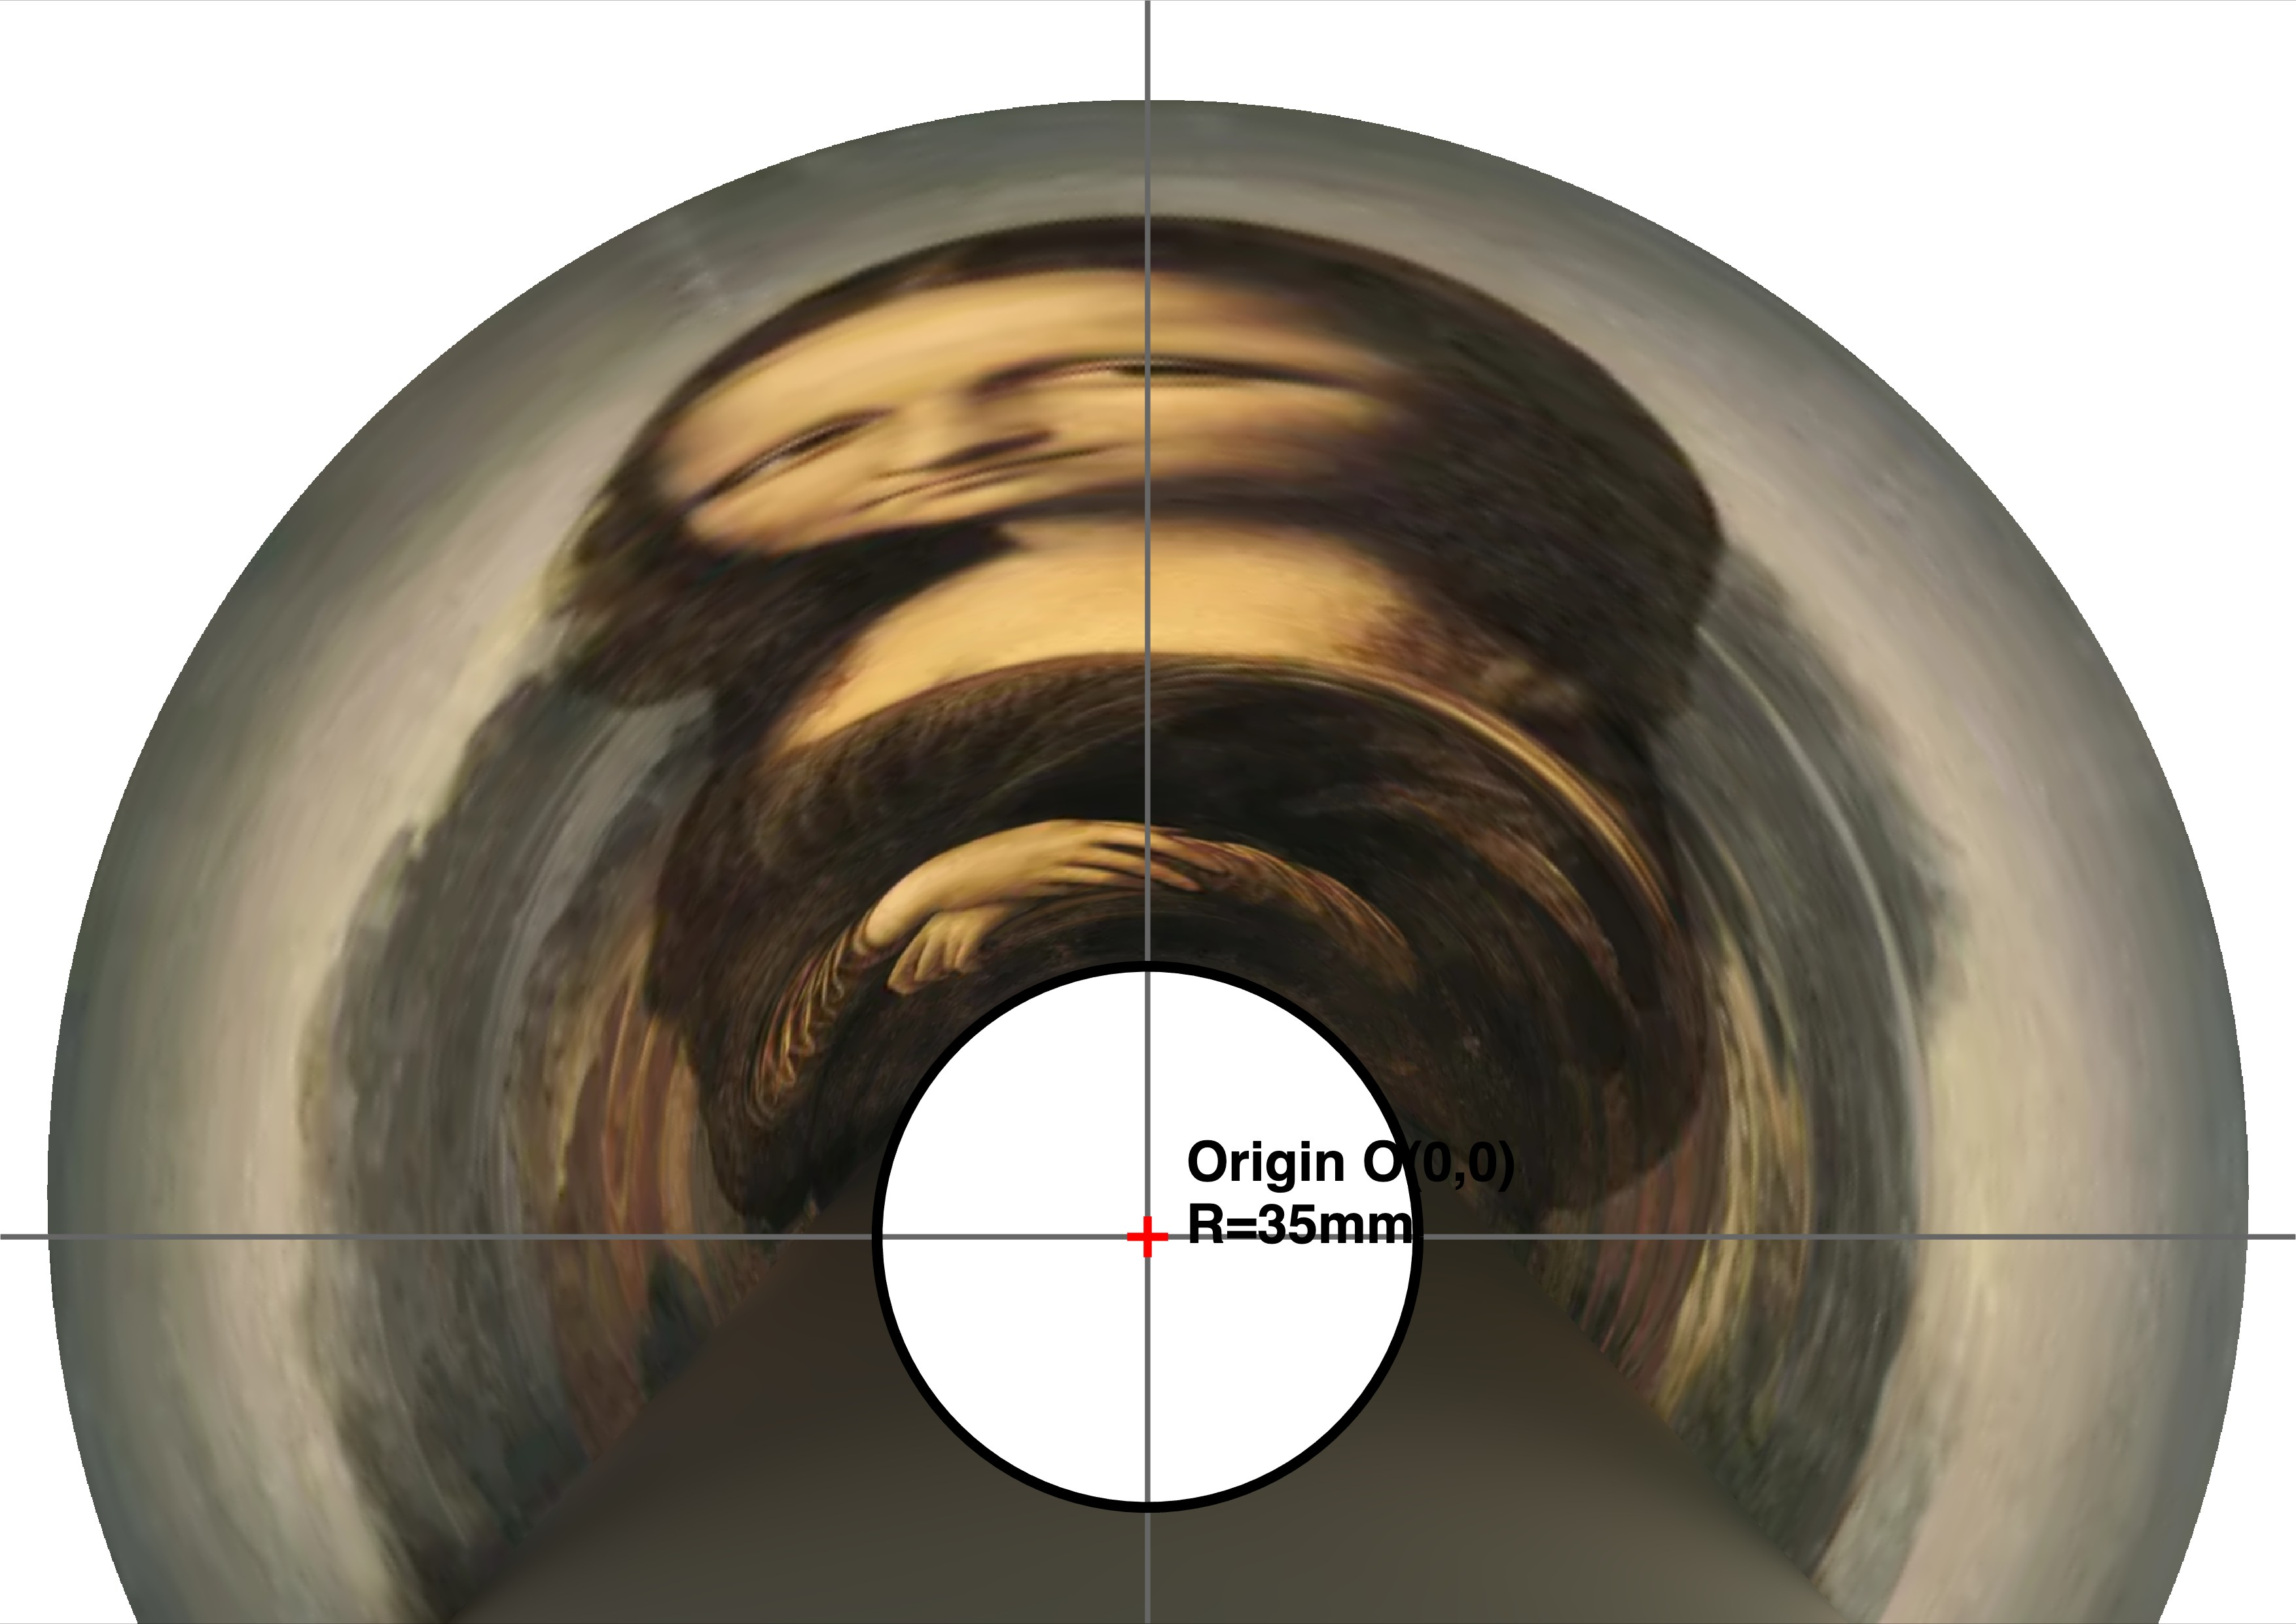
\includegraphics[width=0.46\textwidth]{../../outputs/figures/draft/p3_2D_matlab.jpg}
\includegraphics[width=0.46\textwidth]{../../outputs/figures/draft/p3_mirror_perspective_from_paper.png}
\caption{蒙娜丽莎案例的纸面畸变图案与柱面观察模拟结果}
\label{fig:q1-monalisa-result}
\end{figure}

数值验证表明,在上述参数下,蒙娜丽莎案例的纸面投影范围约为
\[
u\in[-142.4,142.4]\ \mathrm{mm},\qquad v\in[-76.8,147.2]\ \mathrm{mm}.
\]
当前横向 A4 输出画布取 $u\in[-148.5,148.5]$ mm,$v\in[-50,160]$ mm,故该方案约有 $98.78\%$ 的采样点落入画布范围。局部雅可比行列式的最小值约为
\[
J_{\min}=9.033>0,
\]
说明在 $\Theta=130^\circ$ 下映射仍保持局部单调,未出现自交叠或方向反转。少量超出 $v=-50$ mm 的点主要位于纸面下边界附近,属于增大张角带来的边界代价。

\subsection{案例二:图 4 卡通猫设计方案}

图 4 为卡通猫图像,颜色块面清晰、轮廓相对简单,相比写实肖像对局部形变更具有容忍度。为验证同一几何模型对不同图像类型的适应性,卡通猫案例保持圆柱和观察者参数不变:
\[
R=35\ \mathrm{mm},\qquad D=250\ \mathrm{mm},\qquad z_E=350\ \mathrm{mm},\qquad H=150\ \mathrm{mm}.
\]
考虑到卡通图像纵向细节少、主体近似居中,将镜面有效高度压缩为
\[
z\in[2,90]\ \mathrm{mm},
\]
并同样采用总张角
\[
\Theta=130^\circ.
\]
镜面参数域离散为 $400\times300$ 个采样点。较小的高度区间使纸面投影更紧凑,也为较大张角保留了更充足的 A4 边界余量。

\begin{figure}[htbp]
\centering
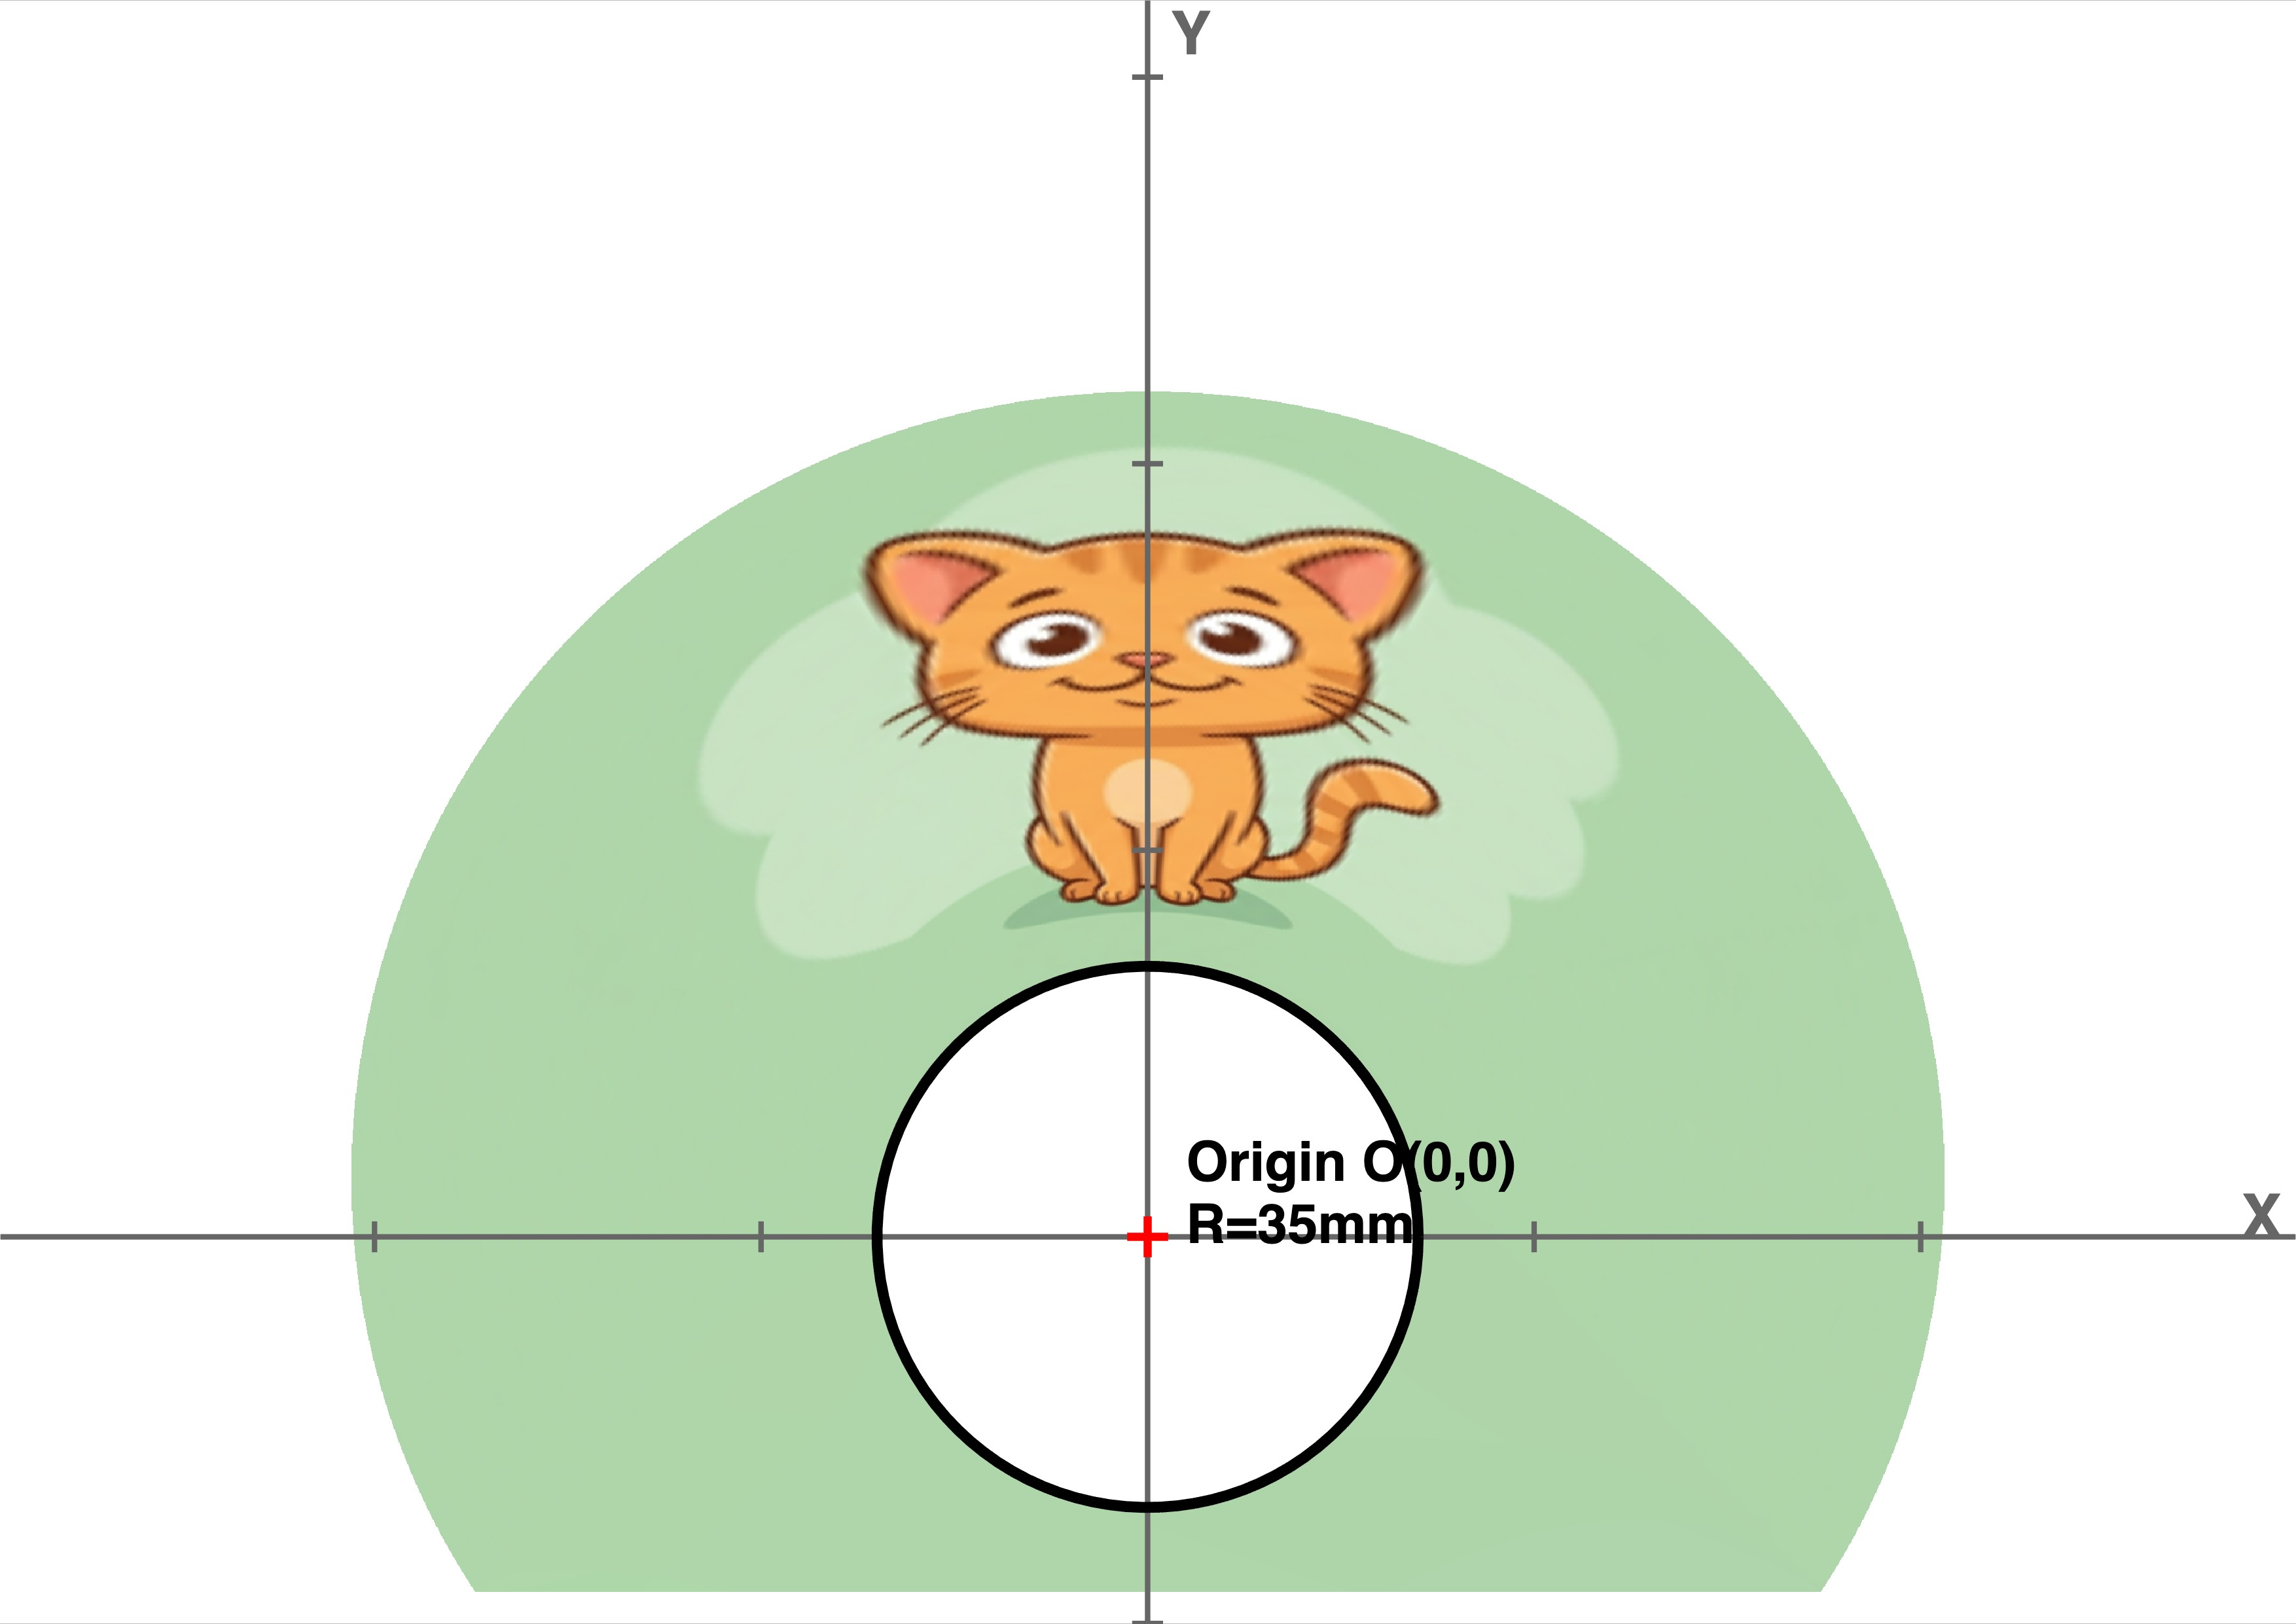
\includegraphics[width=0.46\textwidth]{../../outputs/figures/draft/p4_2D_matlab.jpg}
\includegraphics[width=0.46\textwidth]{../../outputs/figures/draft/p4_mirror_perspective_from_paper.png}
\caption{卡通猫案例的纸面畸变图案与柱面观察模拟结果}
\label{fig:q1-cat-result}
\end{figure}

该案例的纸面投影范围约为
\[
u\in[-103.1,103.1]\ \mathrm{mm},\qquad v\in[-46.0,109.4]\ \mathrm{mm},
\]
完全落入当前横向 A4 画布范围。对应的局部雅可比行列式最小值同样约为
\[
J_{\min}=9.032>0.
\]
因此,卡通猫案例在 $130^\circ$ 张角下既无自交叠,也不存在边界裁切问题,说明较短的高度区间能够显著提升大张角设计的可行性。

\subsection{正向重建验证}

为避免仅凭纸面图案的视觉形态判断方案可行,本文进一步进行正向重建验证。具体做法是:以生成的纯纸面图案 $F(u,v)$ 为输入,对观察者视点 $\mathbf{E}$ 发出的每条视线求其与圆柱面的交点,再利用相同的光学映射反查该镜面点对应的纸面坐标,从 $F$ 中双线性采样得到观察者实际看到的颜色。该过程等价于从纸面图案重新渲染镜面观察图 $\hat{G}$,可检验反问题设计是否在正向成像中恢复目标图案。

为了降低数值渲染误差,正向重建中采用两类输出:
\begin{itemize}
    \item 柱面参数域展开图:直接在 $(\theta,z)$ 规则网格上采样,用于检查图像内容是否完整;
    \item 观察点透视图:从 $\mathbf{E}=(0,250,350)$ mm 处进行透视渲染,并使用 $2\times$ 超采样和 Lanczos 缩放降低边缘锯齿。
\end{itemize}
验证结果显示,两幅目标图像均能在柱面上恢复为可辨识的主体图案。其中蒙娜丽莎案例更接近边界极限,小猫案例则具有更大的边界冗余。由此可见,$90^\circ$ 并非本模型的物理上限,而只是 $\phi\approx2\theta$ 近似解释的高精度范围;在使用完整公式时,$130^\circ$ 张角仍可得到稳定成像。

\begin{table}[htbp]
\centering
\caption{Q1 两个案例的边界与单调性验证}
\label{tab:q1-validation}
\begin{tabular}{lcccc}
\toprule
\textbf{案例} & \textbf{张角} & \textbf{高度区间/mm} & \textbf{A4 内点比例} & \textbf{$J_{\min}$} \\
\midrule
蒙娜丽莎 & $130^\circ$ & $[2,120]$ & $98.78\%$ & $9.033$ \\
卡通猫 & $130^\circ$ & $[2,90]$ & $100.00\%$ & $9.032$ \\
\bottomrule
\end{tabular}
\end{table}

图~\ref{fig:q1-paper-footprint} 给出了两组案例在 $\Theta=130^\circ$ 时的纸面投影足迹。可以看出,两者均呈典型环形扇区分布,圆柱底面对应的圆盘区域被排除在可打印图案之外。蒙娜丽莎案例由于 $z_{\max}=120$ mm,外圈半径更大,其下边界更接近 A4 画布外缘;卡通猫案例高度区间较短,投影区域整体更紧凑。

\begin{figure}[htbp]
\centering
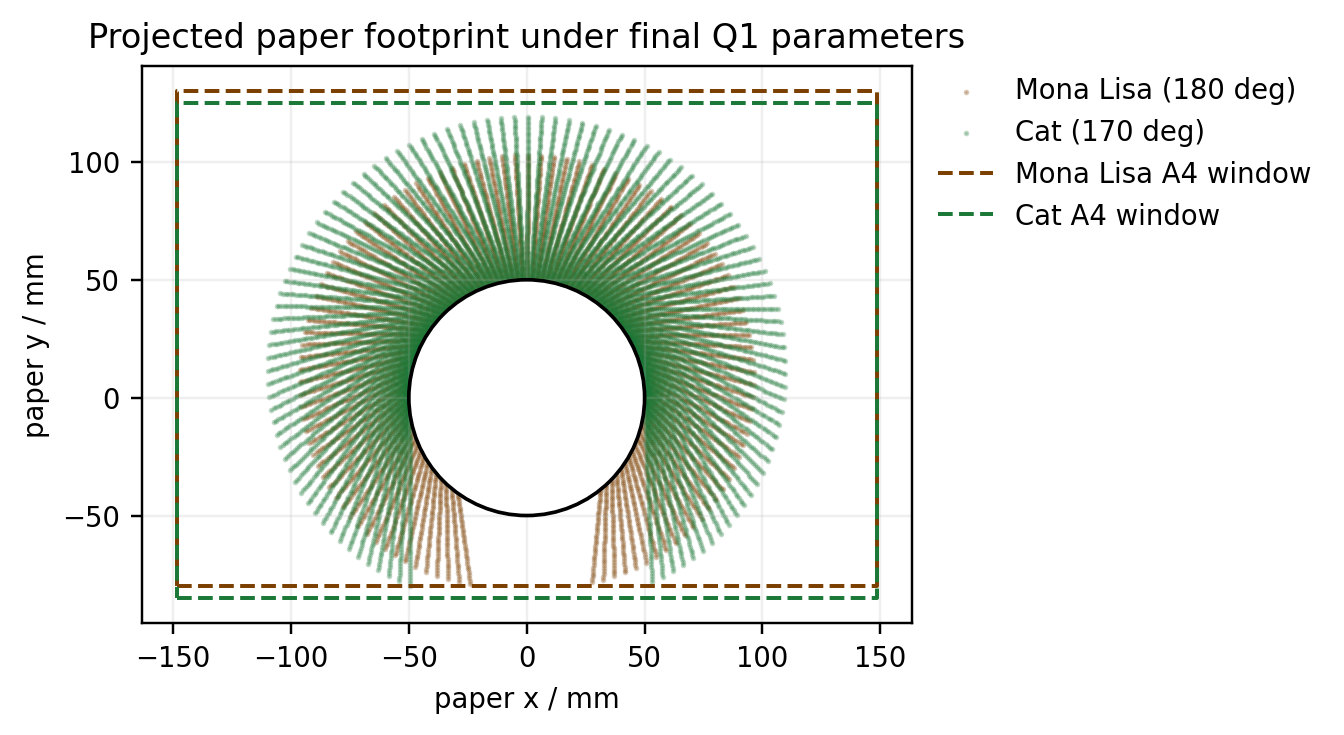
\includegraphics[width=0.72\textwidth]{../../outputs/figures/draft/q1_paper_footprint.png}
\caption{Q1 两个案例在纸面上的投影足迹与 A4 边界关系}
\label{fig:q1-paper-footprint}
\end{figure}

进一步地,图~\ref{fig:q1-jacobian} 给出了局部雅可比行列式在镜面参数域 $(\theta,z)$ 上的分布。两幅热力图均未出现非正区域,说明当前参数下映射保持局部单调。热力图还表明畸变强度主要随高度 $z$ 变化:靠近底部时纸面压缩/拉伸更强,随 $z$ 增大逐渐趋于平缓。这一现象解释了为何 $z_{\max}$ 是影响纸面边界和图像稳定性的关键参数。

\begin{figure}[htbp]
\centering
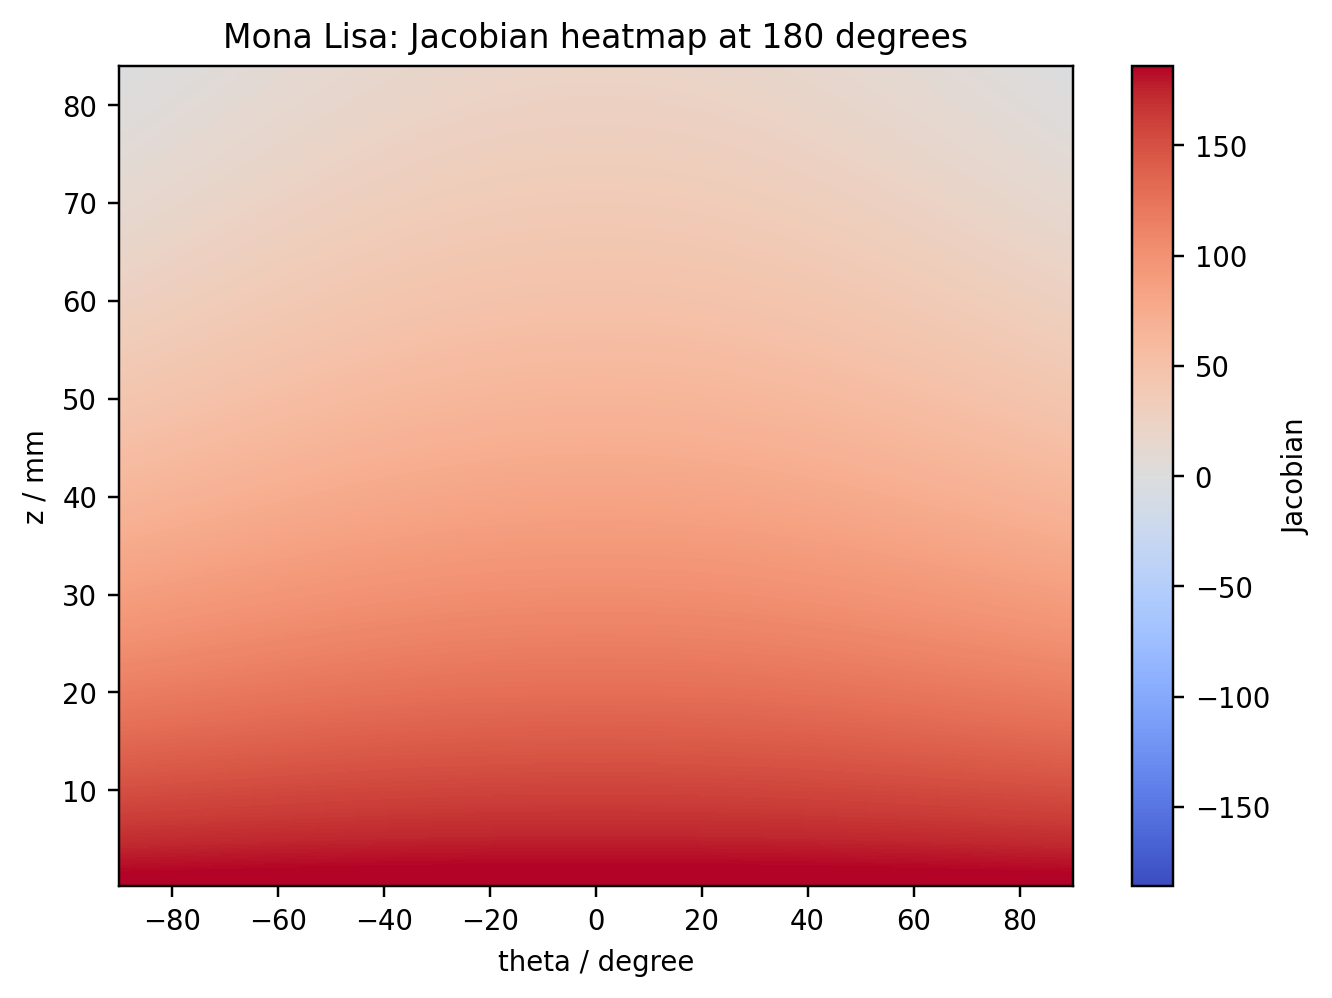
\includegraphics[width=0.47\textwidth]{../../outputs/figures/draft/q1_jacobian_mona_lisa.png}
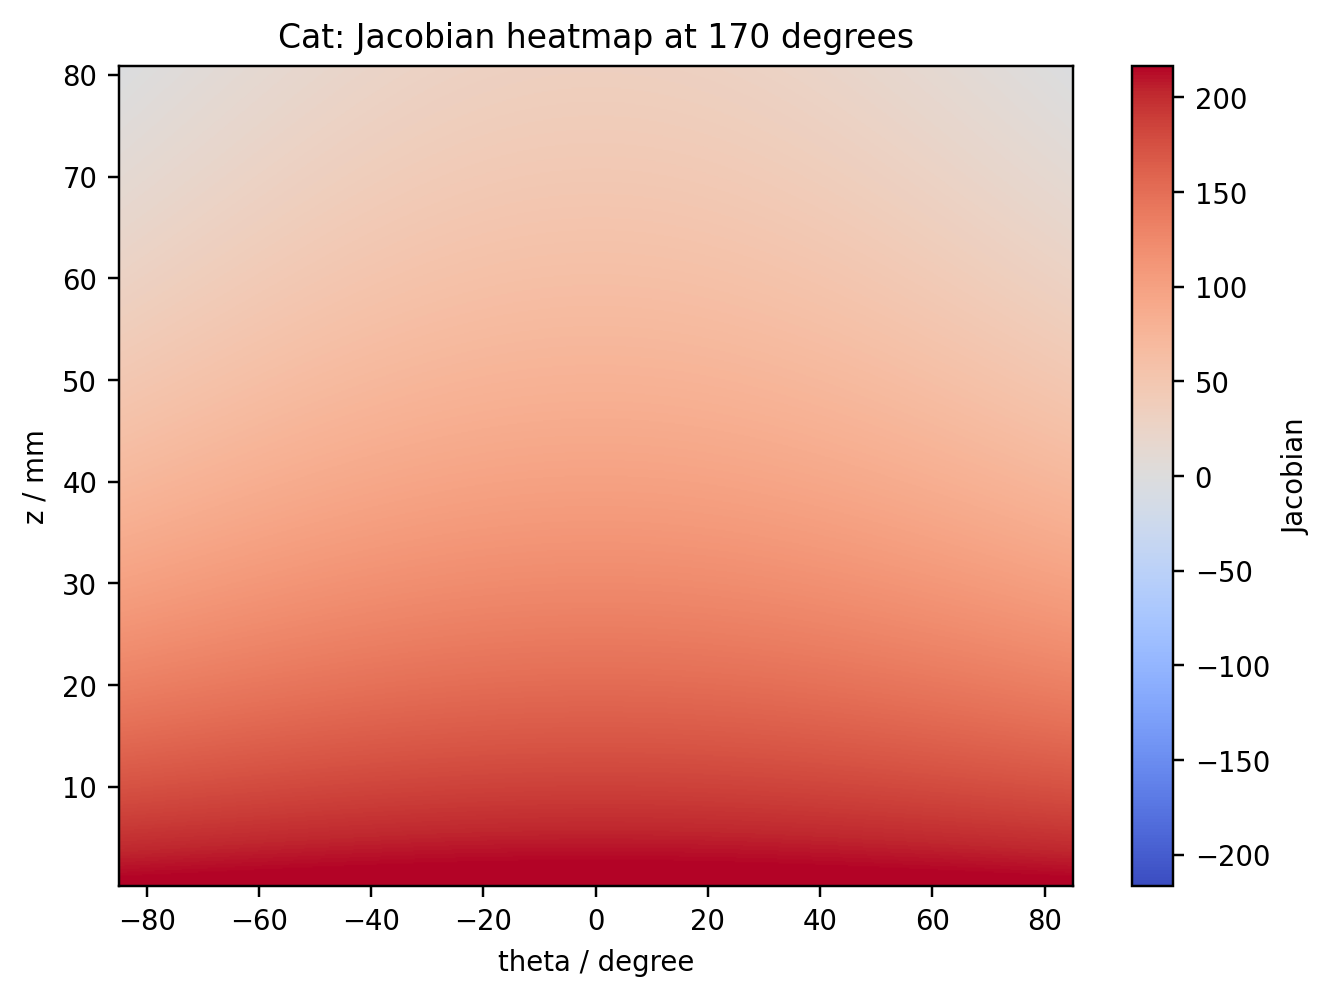
\includegraphics[width=0.47\textwidth]{../../outputs/figures/draft/q1_jacobian_cat.png}
\caption{蒙娜丽莎与卡通猫案例的雅可比行列式热力图}
\label{fig:q1-jacobian}
\end{figure}

\subsection{参数敏感性分析}

从公式
\[
\rho(\theta,z)=\sqrt{\alpha^2R^2+\beta^2D^2+2\alpha\beta RD\cos\theta}
\]
可以看出,$R$、$D$、$z_E$ 与 $z_{\max}$ 会共同决定纸面图案的径向跨度和横向张开程度。固定其余参数时:
\begin{itemize}
    \item 增大 $R$ 会增大圆柱遮挡圆盘,并改变内圈附近投影形态;过大的 $R$ 会压缩纸面可用空间。
    \item 增大 $D$ 使观察光线更接近平行,切向拉伸减弱,纸面图案两翼向中部收缩。
    \item 增大 $z_{\max}$ 会显著提高外圈投影半径,是导致 A4 边界溢出的主要因素。
    \item 增大总张角 $\Theta$ 会优先扩大纸面下边界和两侧边缘处的投影范围,因此需结合 A4 边界和雅可比行列式共同判断。
\end{itemize}
对当前参数进行角度扫描可知,$120^\circ$ 到 $130^\circ$ 仍保持单调性;当张角继续增至 $140^\circ$ 以上时,蒙娜丽莎案例的 A4 下边界裁切明显增加。接近 $180^\circ$ 时,数值雅可比行列式出现负值,说明局部映射开始发生方向反转。因此,本文选择 $130^\circ$ 作为兼顾镜面覆盖范围与边界稳定性的折中方案。

\begin{figure}[htbp]
\centering
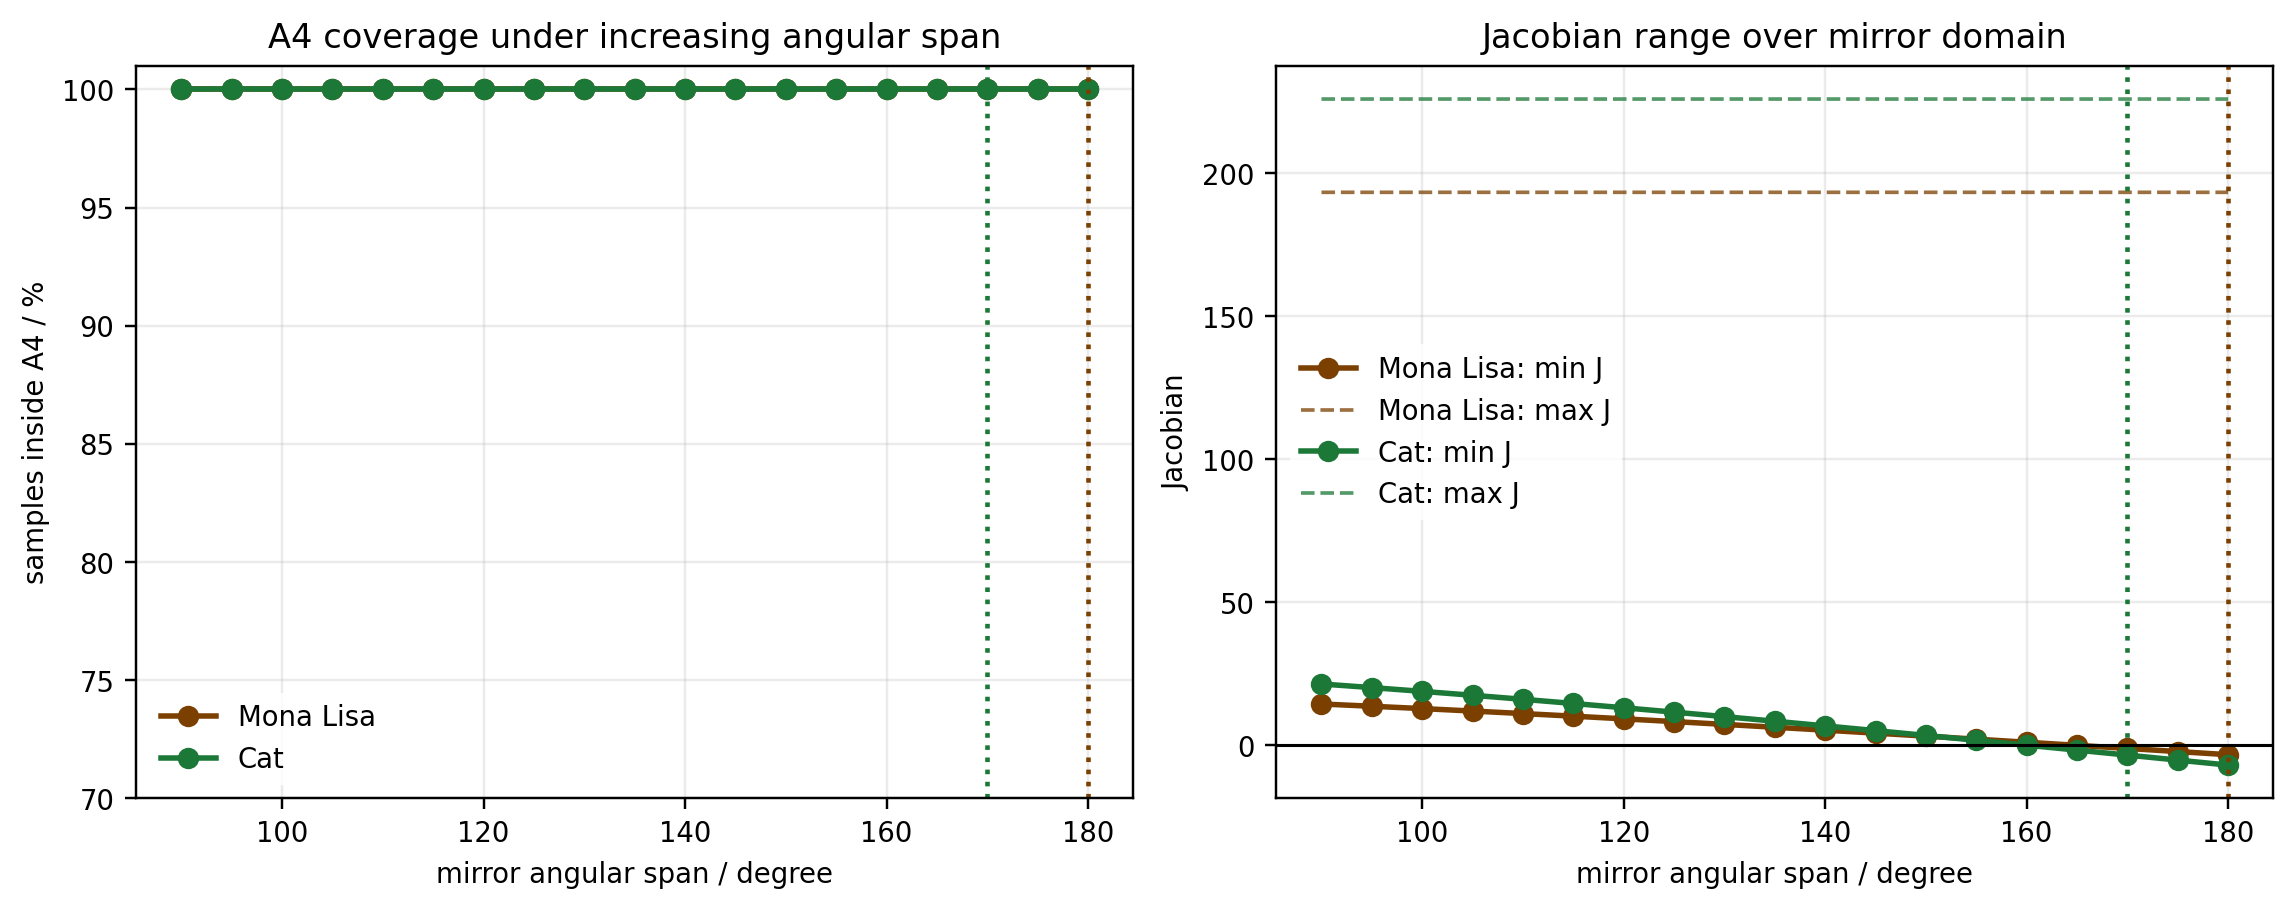
\includegraphics[width=0.92\textwidth]{../../outputs/figures/draft/q1_angle_scan.png}
\caption{总张角变化对 A4 覆盖率与局部单调性的影响}
\label{fig:q1-angle-scan}
\end{figure}

\subsection{本章小结}

本章建立了由目标镜面图案反求纸面畸变图案的完整流程。通过镜面参数化、反射光线映射、散点插值和 A4 边界验证,分别完成了蒙娜丽莎与卡通猫两组案例设计。数值结果表明,在 $R=35$ mm,$D=250$ mm,$z_E=350$ mm 的条件下,两组方案在 $130^\circ$ 张角下均保持局部单调成像;其中卡通猫完全落入 A4 画布,蒙娜丽莎仅存在少量边界裁切。正向重建图进一步验证了纸面图案能够在圆柱镜中恢复目标图像,说明本文模型可用于实际的柱面反射变形艺术设计。

\section{Q2:纸面也有意义的作品设计}
\subsection{子问题分析}
把 Q2 拆成两种情形:(a) 双自由、(b) 镜面受约束。指出自由度差异。

\subsection{对称性理论:纸面-镜面图案的频域对应}
A 核心贡献。FFT 证明:纸面极坐标 FFT 的径向/角向能量 $\leftrightarrow$ 镜面直角坐标 FFT 的横向/纵向能量。由此得到"纸面放射$\rightarrow$镜面竖条纹""纸面环形$\rightarrow$镜面横条纹"的判据。

\subsection{子问题 (a):纸面与镜面均有意义、相互独立}
策略:在对称性兼容的候选纸面图案库中筛选。

\subsubsection{候选图案库}
曼陀罗、对数螺旋、向日葵螺旋、Voronoi、分形树等 10 种。

\subsubsection{实验结果与筛选}
展示 2-3 组"两边都好看"的作品图。

\subsection{子问题 (b):指定镜面图案、纸面也有意义}
策略:简化镜面图案 + 可视盲区利用 + 艺术再解读。

\subsubsection{可视盲区的几何推导}
给出纸面上反射线无法到达观察者的区域公式。

\subsubsection{实施方案}
在必要纸面区域反推畸变图案,在盲区和空白区域独立创作。

\subsubsection{案例展示}
1-2 组完整作品,标明哪部分是反射有效区、哪部分是独立创作区。

\subsection{本章小结}

\section{Q3:双约束下的兼容性理论}
\subsection{问题本质与不可行性分析}
解释为什么"任意两张图"一般不兼容:$T^{-1}(G)$ 唯一确定,与独立给定的 $F$ 同时相等的概率为零。艺术加工的数学含义 = 容忍度。

\subsection{兼容性条件的数学定义}
本文最大创新点。列 5 条可计算判据:

\subsubsection{拓扑兼容}
连通分量数差 $\leq \varepsilon_1$。

\subsubsection{尺度兼容}
镜面每行对应纸面环形面积 $\rightarrow$ 细节密度上界。

\subsubsection{几何对称兼容}
极坐标 FFT 主频 vs 直角坐标 FFT 主频相关系数 $\geq \varepsilon_2$。

\subsubsection{可视区域兼容}
$G$ 支撑集必须落在 $T(\mathcal{I}_{vis})$ 内。

\subsubsection{艺术容忍度}
差异图 $D$ 的高误差区域占比 + 纹理复杂度。

\subsection{构造性判决算法}
伪代码:5 步兼容性检查 $\rightarrow$ 差异图计算 $\rightarrow$ 装饰填充 $\rightarrow$ 可行性得分。配算法流程图。

\subsection{案例一:可行设计}
选一对满足判据的 $F$、$G$,跑算法,展示最终作品 + 各项得分。

\subsection{案例二:不可行反例}
选一对故意违反某条判据的 $F$、$G$(比如蒙娜丽莎 + 小猫),展示算法判决为不可行 + 定量分析哪条判据失败。

\subsection{本章小结}

\section{模型评价与推广}
\subsection{模型优点}
1-2 段。精确、通用、可计算、首次系统化兼容性理论等。

\subsection{模型不足}
坦诚列。未考虑镜面厚度/折射、未考虑二次反射、未考虑观察者双眼视差、兼容性阈值 $\varepsilon$ 需经验标定等。

\subsection{模型推广}
推广到圆锥镜、自由曲面镜;推广到动态 anamorphosis(Luycho Locomotion 系列);推广到 AR/VR 场景。

\section{结论}
一页以内。Q1/Q2/Q3 各一段总结最核心的贡献。最后一句点出艺术+数学交叉的价值。

\section*{参考文献}
5-8 篇核心文献:Hunt 2000 AJP、Spickler \& Bergner 2011、Nicéron 1638、Geng et al. CVPR 2024、Luycho 公开资料等。

\appendix
\section{反射映射完整推导}
2.4 节的详细展开。

\section{核心代码清单}
渲染管线、Q3 算法、每个文件加注释头。

\section{实验参数记录表}
experiments.md 整理版。

\end{document}
